\begin{fact} \label{iso-rect}
	Considérons tous les rectangles de périmètre fixé $p$. Parmi tous ces rectangles, un seul est d'aire maximale, c'est le carré de côté $c = \num{.25} p$.
\end{fact}


\begin{proof}
	Voici une preuve géométrique élémentaire s'appuyant sur le dessin suivant où les rectangles $1$, $2$ et $3$ sont isométriques au rectangle étudié de dimension $L \times \ell$.

	\begin{center}
		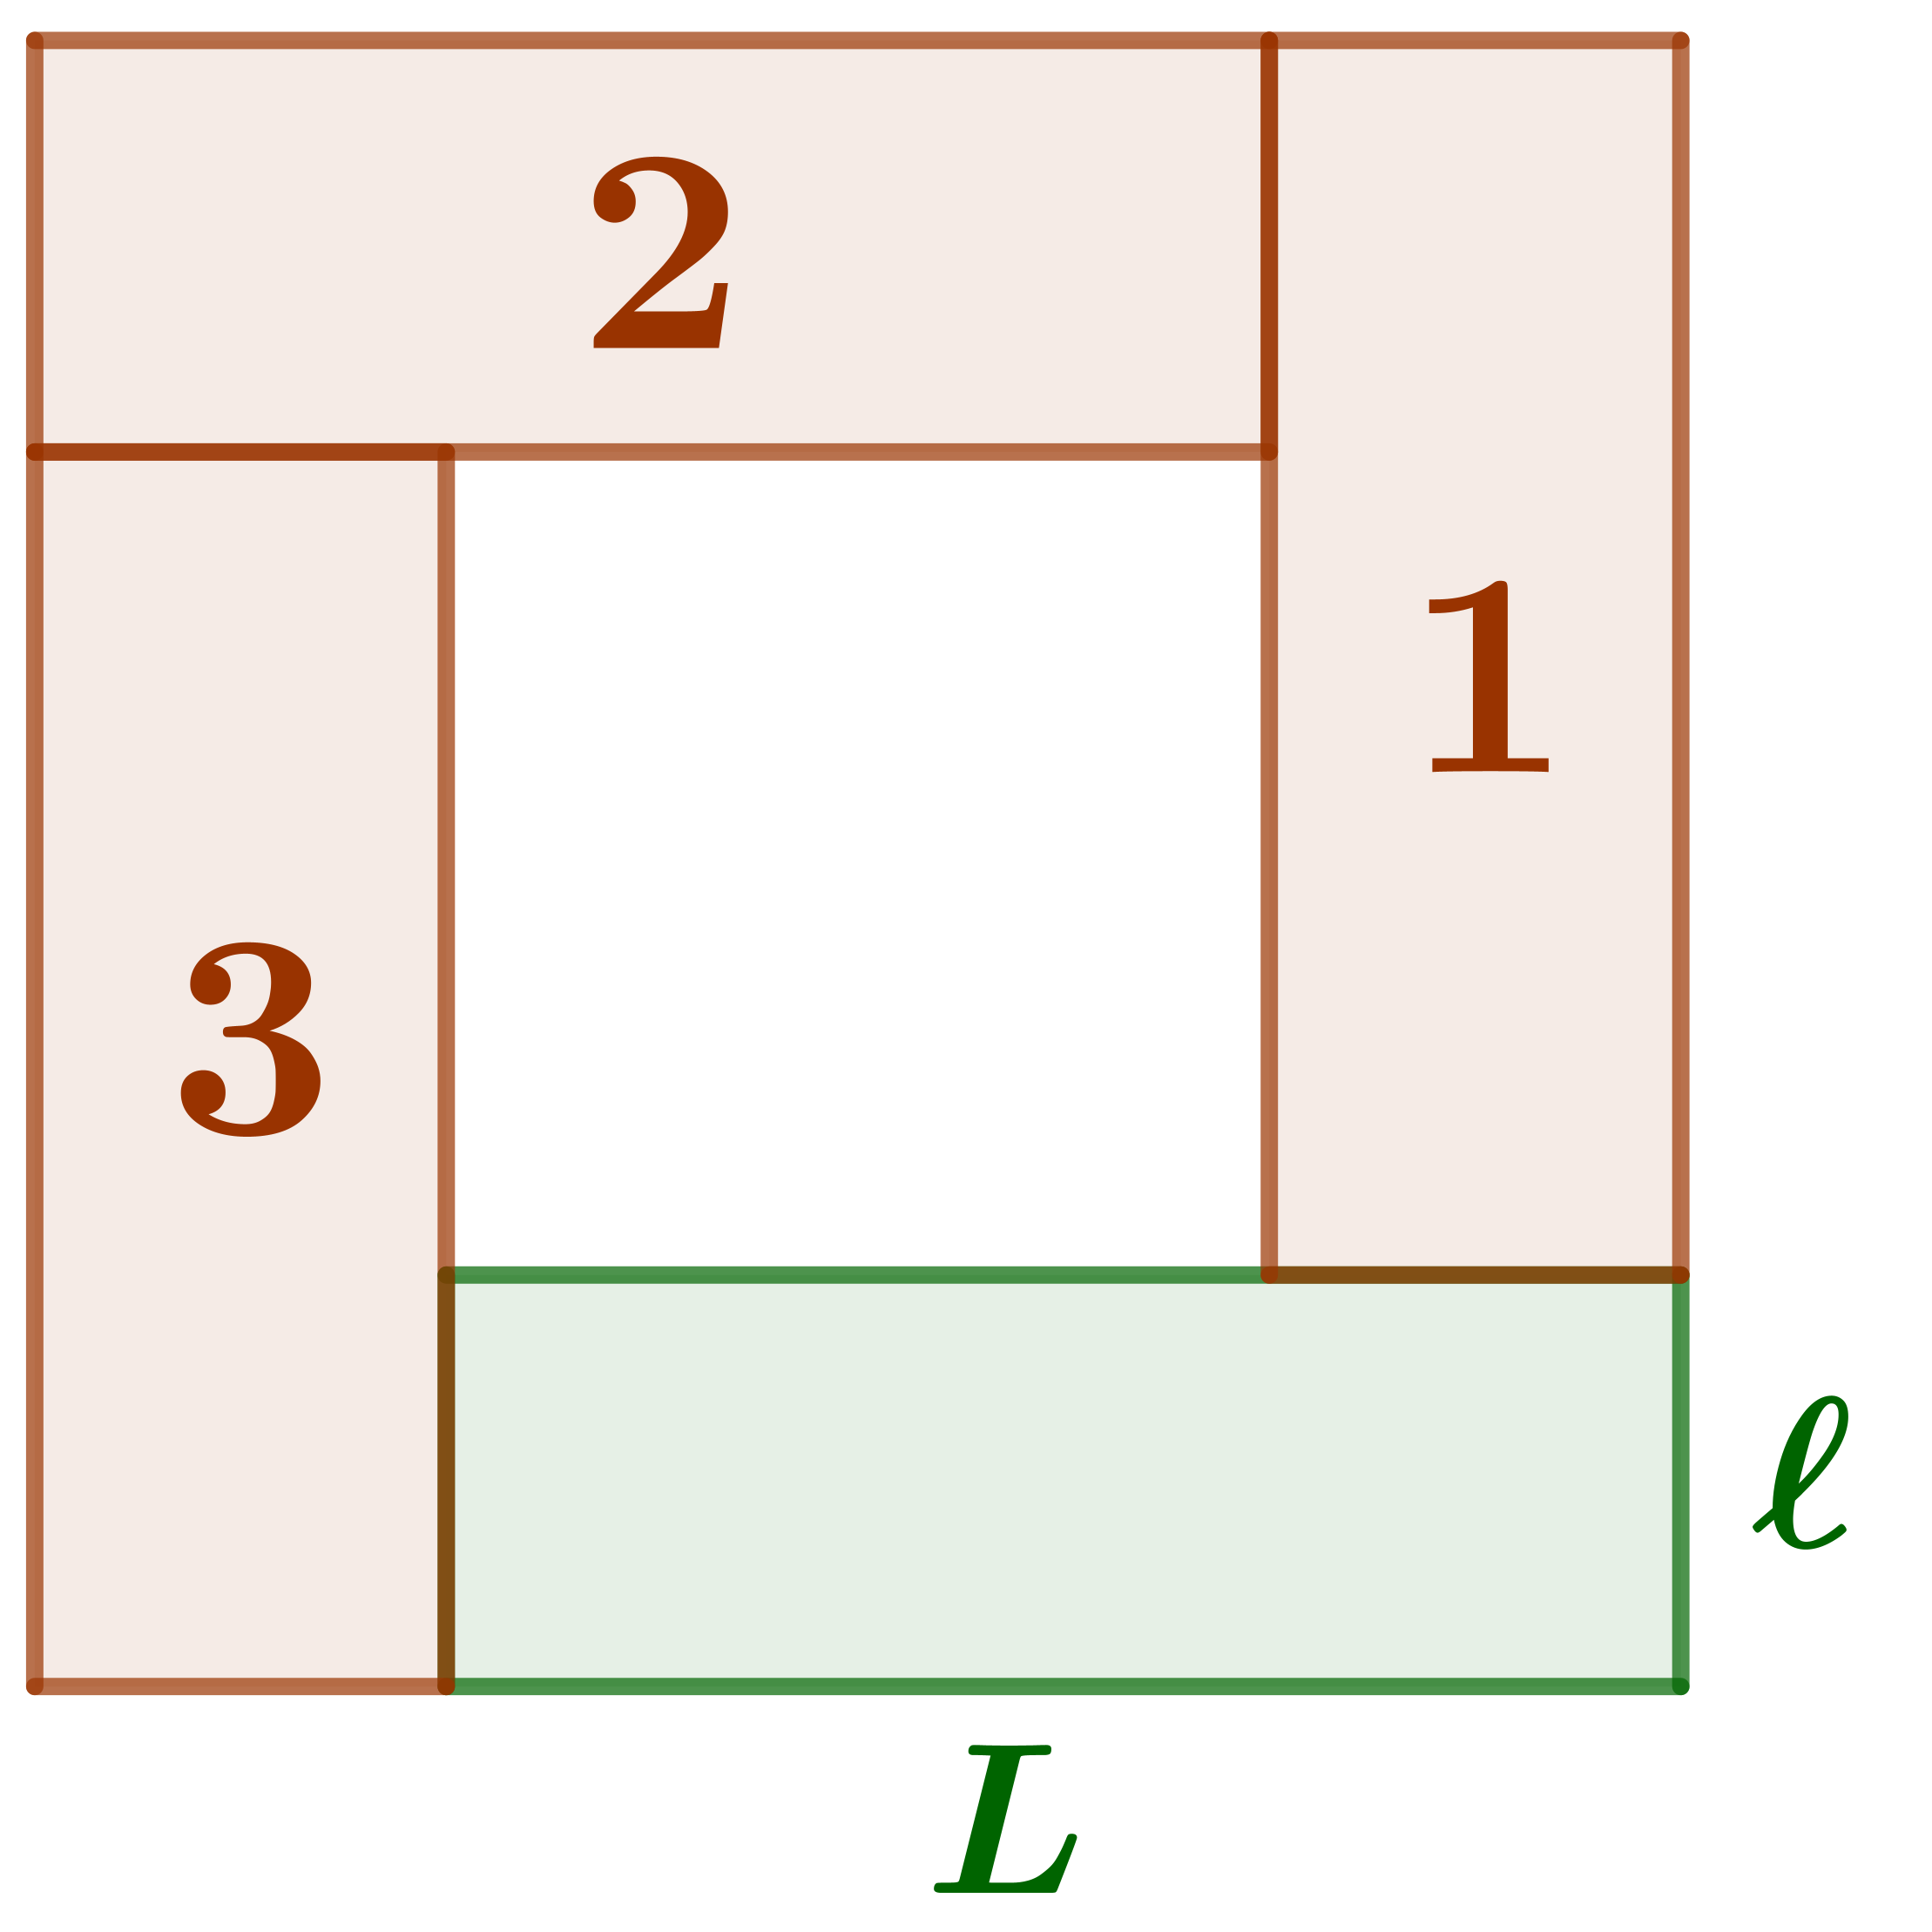
\includegraphics[scale=.4]{content/rectangle/rect-2-square.png}
	\end{center}
	
	Le raisonnement tient alors aux constations suivantes accessibles à un collégien.
	%
	\begin{enumerate}
		\item Le grand carré a une aire $(L + \ell)^2$ supérieure ou égale à $4 L \ell$, et ceci strictement si le rectangle initial n'est pas un carré.

		\item Le grand carré a un périmètre égal à $4 (L + \ell)$.

		\item Une homothétie de rapport \num{.5} donne un carré 
		de périmètre $\num{.5} \times 4 (L + \ell) = 2 (L + \ell)$,
		et d'aire supérieure ou égale à $\num{.5}^2 \times 4 L \ell =  L \ell$, avec inégalité stricte si le rectangle initial n'est pas un carré.
	\end{enumerate}
	
	Donc, parmi tous les rectangles de périmètre $p = 2 (L + \ell)$ et d'aire $L \ell$, le carré est celui d'aire maximale. Joli! Non?
\end{proof}


% ----------------------- %


\begin{remark}
	Une preuve courante consiste à exprimer l'aire du rectangle comme polynôme du 2\ieme\ degré en $L$, par exemple: on obtient $L \ell = L (\num{.5} p - L)$ qui est maximale en $L_M = \num{.25} p$ (moyenne des racines), d'où $\ell_M = \num{.25} p = L_M$.
\end{remark}


% ----------------------- %


\begin{remark} \label{ineq-geo-quad-arith}
	Nous avons établi
	$4 L \ell \leq (L + \ell)^2$
	pour $(L ; \ell) \in \big( \RRsp \big)^2$.
	Ceci permet de comparer les moyennes arithmétique $\frac12 (L + \ell)$, géométrique $\sqrt{L \ell}$ et quadratique $\sqrt{\frac12 (L^2 + \ell^2)}$ d'ordre $2$.
	Voici comment faire.
	%
	\begin{itemize}
		\item L'application de la racine carrée donne
		$2 \sqrt{L \ell} \leq L + \ell$, puis 
		$\sqrt{L \ell} \leq \frac12 (L + \ell)$.
		
		\item Un simple développement fournit $2 L \ell \leq L^2 + \ell^2$, puis
    	$\sqrt{L \ell} \leq \sqrt{\frac12 (L^2 + \ell^2)}$.
		
		\item On peut faire mieux en notant que $2 L \ell \leq L^2 + \ell^2$ donne
		$L^2 + \ell^2 + 2 L \ell \leq 2 (L^2 + \ell^2)$, puis
		$\frac14 (L + \ell)^2 \leq \frac12 (L^2 + \ell^2)$, et enfin 
		$\frac12 (L + \ell) \leq \sqrt{\frac12 (L^2 + \ell^2)}$.
	\end{itemize}
	
	En résumé,
	$\sqrt{L \ell} \leq \frac12 (L + \ell) \leq \sqrt{\frac12 (L^2 + \ell^2)}$
	pour $(L ; \ell) \in \big( \RRsp \big)^2$.
	%
	Ces inégalités se généralisent à l'ordre $n$ grâce à l'algèbre, ou l'analyse.
\end{remark}
